\documentclass[12pt,a4paper]{article}
\usepackage{fontspec}
\usepackage{polyglossia}
\setdefaultlanguage{russian}
\setmainfont{STIX Two Text}[AutoFakeBold=1.5]
\setmonofont{Menlo}
\newfontfamily\cyrillicfonttt{Menlo}
\usepackage[a4paper,margin=2cm]{geometry}
\usepackage{graphicx,longtable,tabularx,array,booktabs}
\usepackage{float,caption,enumitem,pdflscape,xurl,listings,tikz}
\usepackage{hyperref,etoolbox}
\usetikzlibrary{positioning,arrows.meta}
\hypersetup{colorlinks=true,linkcolor=blue,urlcolor=blue}
\lstset{basicstyle=\ttfamily\footnotesize,breaklines=true,columns=fullflexible,frame=single,keepspaces=true,showstringspaces=false}
\setlength{\parindent}{1.25cm}
\setlength{\parskip}{0.25em}
\setlength{\emergencystretch}{2em}
\renewcommand{\arraystretch}{1.16}
\setlist{nosep,leftmargin=1.5em}
\AtBeginEnvironment{longtable}{\small}
\begin{document}
\begin{titlepage}
\centering
\vspace*{1.5cm}
Практическая работа\\[3.2cm]
{\Large\bfseries Отчёт по практической работе № 8}\\[0.6cm]
{\large Реализация ролевого управления доступом}\\[3.4cm]
\begin{tabular}{p{5.2cm}p{9cm}}
Дисциплина: & Основы разработки защищённого программного обеспечения и компьютерных сетей \\
Вариант: & 19 — Система учёта транспортных средств организации \\
Исходная версия: & v0.7 \\
Версия работы: & v0.8 \\
Студент: & Мостовая Полина Андреевна \\
Группа: & ИУСбд-02-23 \\
\end{tabular}
\vfill
2026
\end{titlepage}

\pagenumbering{arabic}
\tableofcontents
\clearpage

\section{Тема, цель и среда}
Тема — реализация ролевого управления доступом (RBAC) в сквозном проекте учёта транспортных средств. Цель — связать подтверждённый сеанс v0.7 с текущей серверной ролью, проверить разрешение и принадлежность заявки, а при запрете сохранить защищённые данные неизменными. Дополнительный вариант 19 — повторное открытие закрытой заявки в области Б, то есть только в подразделении specialist.

Работа продолжает локальный проект v0.7. В v0.5 реализованы разбор JSON и \texttt{ValidatedRequest}; в v0.6 — \texttt{RequestRepository}, SQLite и \texttt{FileStore}; в v0.7 — \texttt{AuthService}, парольные проверочные значения и серверные сеансы. Существующая модель предметных операций автопарка (\texttt{driver}, \texttt{dispatcher}, \texttt{manager}, \texttt{security\_admin}) сохранена отдельно. Роли \texttt{user}, \texttt{operator}, \texttt{admin}, \texttt{specialist} применяются только к учебным заявкам.

Методичка №8 содержит 14 страниц; требования адаптированы к фактическим модулям. В репозитории нет сохранённой рабочей SQLite-БД. Текущая среда разработки: macOS, Python 3.12.14 в \texttt{.venv}, SQLite стандартной библиотеки. Проект не содержит сетевого API.

\section{Соответствие v0.5--v0.7}
\begin{longtable}{p{2.1cm}p{5.2cm}p{7.3cm}}
\toprule Предыдущая работа & Имеющийся компонент & Использование в v0.8 \\
\midrule\endhead
v0.5 & \texttt{validate\_request} & Контракт содержимого заявки передаётся в защищённый сервис; \texttt{owner\_id}, роль, active и department не входят в клиентские поля. \\
v0.6 & \texttt{RequestRepository}, таблица заявок, \texttt{FileStore} & Существующая таблица расширяется без удаления полей; сохраняются категория, приоритет, описание и ключи вложений. \\
v0.7 & \texttt{AuthService.resolve} & Адаптер возвращает только серверный ID пользователя для действующего сеанса; парольная проверка не дублируется. \\
v0.4 & \texttt{Principal}, роли автопарка & Старая in-memory RBAC-модель остаётся отдельной; названия ролей и политика не меняются. \\
\bottomrule
\end{longtable}

\section{Модель и матрица доступа}
RBAC связывает роль с разрешёнными операциями; он не освобождает от проверки конкретного объекта [2, 5]. В этой учебной модели у пользователя одна текущая роль без наследования. Для \texttt{user} разрешённое \texttt{request.read} дополняется условием \texttt{requests.owner\_id = users.id}. Для неизвестной роли и операции применяется отказ по умолчанию. Сервер не принимает идентификатор субъекта, роль или атрибут подразделения из заявки [1, 3].

\begin{longtable}{p{5.3cm}p{1.8cm}p{1.8cm}p{1.8cm}p{2.5cm}}
\toprule Операция & user & operator & admin & specialist \\
\midrule\endhead
Создать заявку & Да & Нет & Нет & Нет \\
Читать заявку & Только свою & Все учебного контура & Нет & Нет \\
Закрыть \texttt{new → closed} & Нет & Да & Нет & Нет \\
Назначить обычную роль & Нет & Нет & Другому обычному пользователю & Нет \\
Повторно открыть \texttt{closed → new} & Нет & Нет & Нет & Только своё подразделение \\
Назначить/изменить admin & Нет & Нет & Нет & Нет \\
Неизвестное действие & Запрет & Запрет & Запрет & Запрет \\
\bottomrule
\end{longtable}

admin управляет только ролями и не получает права чтения заявок. specialist не получает разрешений operator или admin. Открытая регистрация назначает \texttt{user}; первичная административная запись — доверенная локальная подготовка, вне публичной регистрации.

\section{Интеграция с аутентификацией и SQLite}
AccessService вызывает \texttt{AuthService.resolve} и получает только серверный ID для действующего сеанса. Клиент не может передать ID вместо токена. При каждом вызове в общей SQLite-БД читаются текущие \texttt{active}, \texttt{role} и \texttt{department\_id}. Роль не встраивается в сессию, поэтому назначение или отзыв применяется при следующем запросе с прежним действующим токеном. Отсутствующая, ошибочная, отозванная или истёкшая сессия и отключённый аккаунт закрывают доступ.

Миграция \texttt{AccessService.initialize(path)} повторно запускает инициализацию пользователей и заявок в одном файле. В v0.7 таблица \texttt{users} получает отсутствующие \texttt{role} (default \texttt{user}) и \texttt{department\_id}; таблица \texttt{requests} получает \texttt{owner\_id}, \texttt{status}, \texttt{department\_id}. Для прежних заявок без владельца/отдела атрибуты остаются \texttt{NULL}, состояние — \texttt{legacy}. Старые парольные хеши, соли, rounds, recovery-хеши, сеансы и прежние поля заявок не пересоздаются. Миграционный тест проверяет совпадение синтетических данных и идемпотентность.

В checkout нет пользовательских файлов SQLite, которые требовали бы объединения. Сервисы в интегрированном контуре должны получить один путь. Если фактические заполненные файлы существуют отдельно, их автоматическое слияние не реализовано: нужна резервная копия и отдельная контролируемая миграция, до неё нельзя заявлять единый атомарный контур.

\section{Транзакционная последовательность}
\begin{figure}[H]
\centering
\begin{tikzpicture}[node distance=7mm and 8mm,box/.style={draw,rounded corners,align=center,text width=2.45cm,minimum height=11mm,font=\small},arrow/.style={-{Stealth},thick}]
\node[box] (client) {Токен и объект\\недоверенный ввод};
\node[box,right=of client] (auth) {AuthService\\resolve(token)};
\node[box,right=of auth] (uid) {Серверный\\user\_id};
\node[box,below=of uid] (db) {SQLite: active, role,\\owner, department};
\node[box,left=of db] (policy) {Разрешение\\и область объекта};
\node[box,left=of policy] (result) {Операция\\или отказ};
\draw[arrow] (client)--(auth); \draw[arrow] (auth)--(uid); \draw[arrow] (uid)--(db); \draw[arrow] (db)--(policy); \draw[arrow] (policy)--(result);
\end{tikzpicture}
\caption{Подтверждение сеанса и проверка роли/объекта; миграция схемы показана в \texttt{docs/authorization\_flow.mmd}.}
\end{figure}

\texttt{AuthService.resolve} выполняется до \texttt{BEGIN IMMEDIATE}, так как он обновляет \texttt{sessions.last\_seen}. После этого сервис держит одну транзакцию общей БД на чтение роли, проверку объекта и модификацию заявки. Значения SQL передаются параметрами. При исключении выполняется \texttt{ROLLBACK}. Условный \texttt{UPDATE} разрешает только \texttt{new → closed} или \texttt{closed → new} с совпадающим отделом. \texttt{BEGIN IMMEDIATE} сериализует пишущие транзакции и снижает параллелизм SQLite [4]. Отзыв полномочия гарантируется для следующего запроса, но не прерывает уже начатую транзакцию.

\section{Вариант 19: specialist и область Б}
Правило: specialist повторно открывает только заявку со статусом \texttt{closed}, если её серверный непустой \texttt{department\_id} равен текущему серверному отделу пользователя. SQL меняет лишь статус на \texttt{new}. NULL, пустое значение, неизвестная заявка, иной статус и другой отдел запрещают действие. Условие не превращает модель в общий ABAC; это дополнительная проверка области объекта поверх одного разрешения \texttt{request.reopen}.

Схема варианта 19 показывает этот исполняемый порядок проверок: токен, AuthService, транзакция, текущая роль и отдел, заявка и статус, равенство отделов, затем изменение или отказ. Клиентское поле \texttt{department\_id} не читается.

\section{Ключевые фрагменты кода}
Таблица разрешений фиксирована и по умолчанию запрещает неизвестные комбинации:
\begin{lstlisting}[language=Python]
PERMISSIONS = {
    "user": frozenset({"request.create", "request.read"}),
    "operator": frozenset({"request.read", "request.close"}),
    "admin": frozenset({"role.assign"}),
    "specialist": frozenset({"request.reopen"}),
}
\end{lstlisting}

Переоткрытие проверяет атрибуты из доверенных строк и изменяет только подходящий закрытый объект:
\begin{lstlisting}[language=Python]
cursor = db.execute(
    "UPDATE requests SET status = 'new' "
    "WHERE id = ? AND status = 'closed' AND department_id = ?",
    (request_id, department_id),
)
if cursor.rowcount != 1:
    raise AccessDenied("Операция недоступна")
\end{lstlisting}
Полная реализация расположена в \texttt{app/authorization.py}; схема роли/состояния добавлена к прежним таблицам в \texttt{app/auth.py} и \texttt{app/repositories/requests.py}.

\section{Базовые тестовые сценарии}
\begin{longtable}{p{0.7cm}p{7.2cm}p{4.1cm}p{2.2cm}}
\toprule № & Проверка & Ожидаемый результат & Факт \\
\midrule\endhead
1 & Владелец читает собственную заявку & Заявка доступна & Пройдено \\
2 & Владелец запрашивает чужую заявку & Единый отказ, без раскрытия & Пройдено \\
3 & Operator читает контур & Заявка доступна & Пройдено \\
4 & Operator закрывает новую заявку & \texttt{new → closed} & Пройдено \\
5 & User пытается закрыть заявку & Отказ, состояние прежнее & Пройдено \\
6 & Создание заявки владельцем & owner взят из сеанса & Пройдено \\
7 & Подмена \texttt{owner\_id} в интерфейсе & Аргумент не поддержан & Пройдено \\
8 & Admin читает заявку & Отказ & Пройдено \\
9 & Admin назначает operator & Новое право доступно & Пройдено \\
10 & User назначает роль & Отказ без изменений & Пройдено \\
11 & Operator назначает роль & Отказ без изменений & Пройдено \\
12 & Попытка назначить admin & Отказ без изменений & Пройдено \\
13 & Изменение существующей admin-записи & Отказ без изменений & Пройдено \\
14 & Роль оператора отозвана при действующем сеансе & Следующая операция запрещена & Пройдено \\
15 & Неизвестный/отозванный сеанс & Отказ & Пройдено \\
16 & Учётная запись отключена & Отказ & Пройдено \\
17 & Неизвестная роль & Отказ & Пройдено \\
18 & Неизвестное разрешение & Отказ & Пройдено \\
19 & Запрошена отсутствующая заявка & Единый отказ & Пройдено \\
20 & Повторное закрытие & Отказ, запись не меняется & Пройдено \\
\bottomrule
\end{longtable}
Базовые проверки находятся в \texttt{tests/test\_authorization.py}; каждый отказ сравнивает состояние пользователей и заявок до/после.

\section{Дополнительные сценарии варианта 19}
\begin{longtable}{p{0.7cm}p{7.2cm}p{4.1cm}p{2.2cm}}
\toprule № & Проверка & Ожидаемый результат & Факт \\
\midrule\endhead
1 & Specialist A открывает закрытую заявку A & Успешно, только статус меняется & Пройдено \\
2 & Specialist A открывает заявку B & Отказ, запись сохранена & Пройдено \\
3 & У пользователя или заявки нет отдела & Отказ, запись сохранена & Пройдено \\
4 & Роль specialist отозвана без нового входа & Сеанс действителен, операция запрещена & Пройдено \\
5 & Заявка уже имеет \texttt{new} & Отказ без изменений & Пройдено \\
6 & Operator/Admin пытается выполнить reopen & Отказ без изменений & Пройдено \\
7 & Клиент передаёт отдел A для заявки B & Аргумент не поддержан & Пройдено \\
8 & Заявки не существует & Отказ без изменений & Пройдено \\
\bottomrule
\end{longtable}

\section{Интеграционные и регрессионные результаты}
Интеграционные проверки создают пользователей через \path{AuthService} и выполняют парольный вход. Сеансы передаются \path{AccessService}; проверяются доступ к своей и чужой заявке, выдача и отзыв operator с прежним сеансом, отключённая запись, выход и истечение по управляемым часам.

Миграционный тест использует искусственные старые таблицы \path{users}, \path{sessions} и \path{requests}; сравнивает соль, хеши, стоимость KDF, recovery-хеш, сеанс и поля заявки.

В отдельном целевом прогоне три файла — \path{tests/test_authorization.py}, \path{tests/test_variant19.py} и \path{tests/test_authorization_integration.py} — прошли 32 теста: 20 базовых, 8 дополнительных и 4 интеграционные проверки. Отдельный интеграционный файл: 4 пройдены. Полный локальный набор: 181 тест и 9 subtests пройдены. Сквозная демонстрация \path{demo_v08.py --all} завершилась успешно; значения токенов и паролей не выводились. Результат относится к первому проходу и будет повторён перед релизом после добавления снимков.

\section{Обнаруженные ограничения}
В реальном checkout нет файла данных для миграции, поэтому проверялись синтетические прежние схемы. Если у пользователя есть раздельные непустые БД, их содержимое не смешивается автоматически; требуется резервная копия и контролируемый импорт. В \texttt{main.py} нет API/маршрутов заявок, поэтому защита проверена на сервисном интерфейсе и сквозной демонстрации, а не на сетевой точке входа. Это существенно ограничивает утверждение об интеграции с будущим приложением.

Файловая система \texttt{FileStore} не участвует в транзакции SQLite; при ошибке после записи применяется компенсирующее удаление. Транзакционный тест относится к пользователям и заявкам в общем файле. \texttt{BEGIN IMMEDIATE} блокирует конкурирующие записи; отзыв роли не останавливает текущую операцию. Целостность SQLite зависит от доверия к процессу и ОС. Нет полноценного жизненного цикла администраторов, согласования изменений ролей, многофакторной защиты, распределённого хранилища или нескольких ролей у пользователя. RBAC не следует трактовать как общую ABAC-систему.

\section{Остаточные риски}
Кража действующего сеансового токена даёт полномочия до отзыва/истечения. Ошибка доверенного admin может назначить чрезмерную роль. Прямое обращение к \texttt{RequestRepository} из будущей внешней точки входа обойдёт сервисную политику. Неполные legacy-атрибуты закрывают специалисту доступ, однако ручное заполнение с ошибкой способно расширить область. Пишущие транзакции SQLite сериализуются; параллельная операция уже начавшаяся до смены роли может завершиться. Компрометация процесса/БД не устраняется тестами. Эти риски описаны также в \texttt{docs/authorization.md}, \texttt{docs/threat\_model.md} и \texttt{docs/risk\_register.md}.

\section{Ручные скриншоты}
Семь снимков сделаны в Terminal.app и включены в отчёт. На них показаны подтверждение сеанса и текущая роль, чтение собственной заявки и отказ на чужую, функциональные разрешения, отзыв роли при прежнем сеансе, положительные и отрицательные сценарии варианта 19, полный запуск тестов и версия проекта. Вывод команд сверяется с автоматическими проверками; значения токенов и паролей не отображаются.
\begin{figure}[H]
\centering
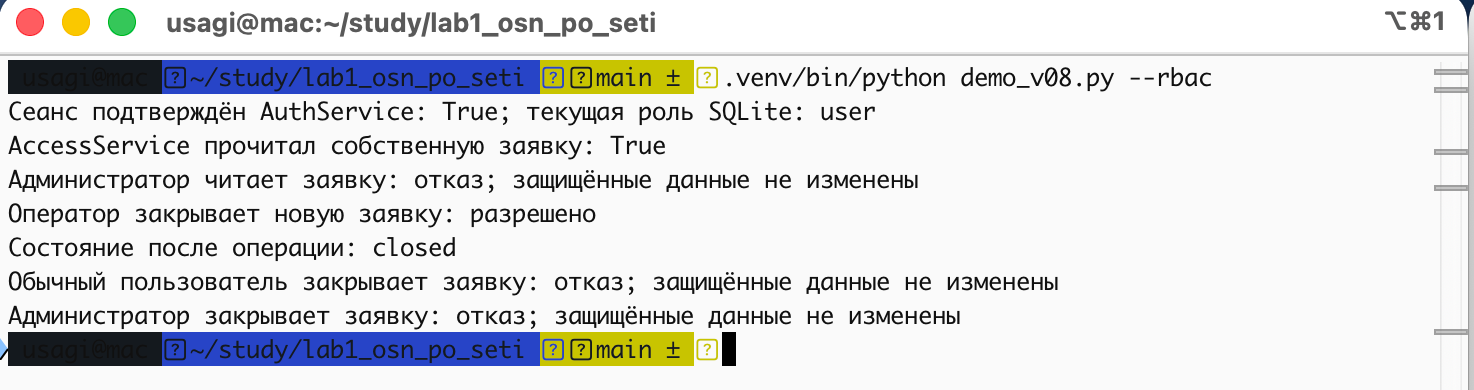
\includegraphics[width=\linewidth,height=5.4cm,keepaspectratio]{reports/lab8/screenshots_manual/lab8_01_identity_role.png}
\caption{Подтверждение сеанса AuthService, текущая роль и доступ к собственной заявке.}
\end{figure}
\begin{figure}[H]
\centering
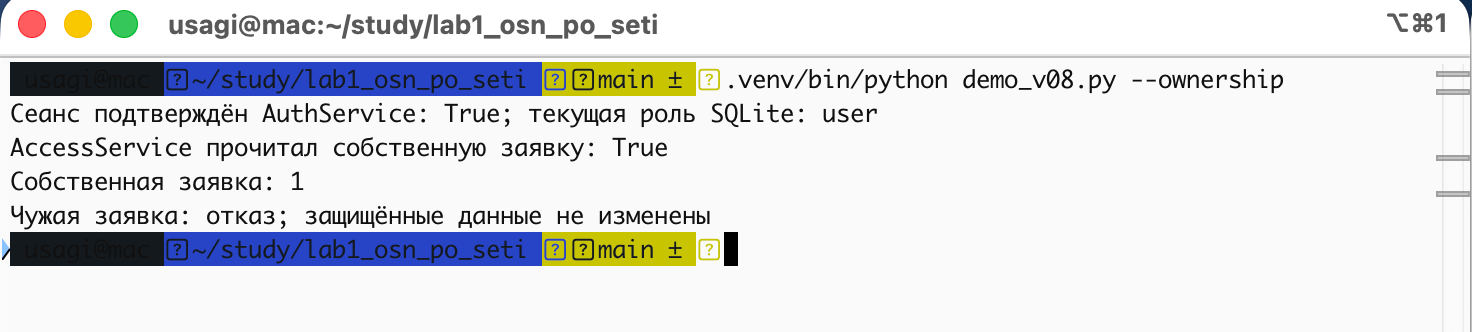
\includegraphics[width=\linewidth,height=5.4cm,keepaspectratio]{reports/lab8/screenshots_manual/lab8_02_ownership.png}
\caption{Объектная авторизация: собственная заявка доступна, чужая отклонена.}
\end{figure}
\begin{figure}[H]
\centering
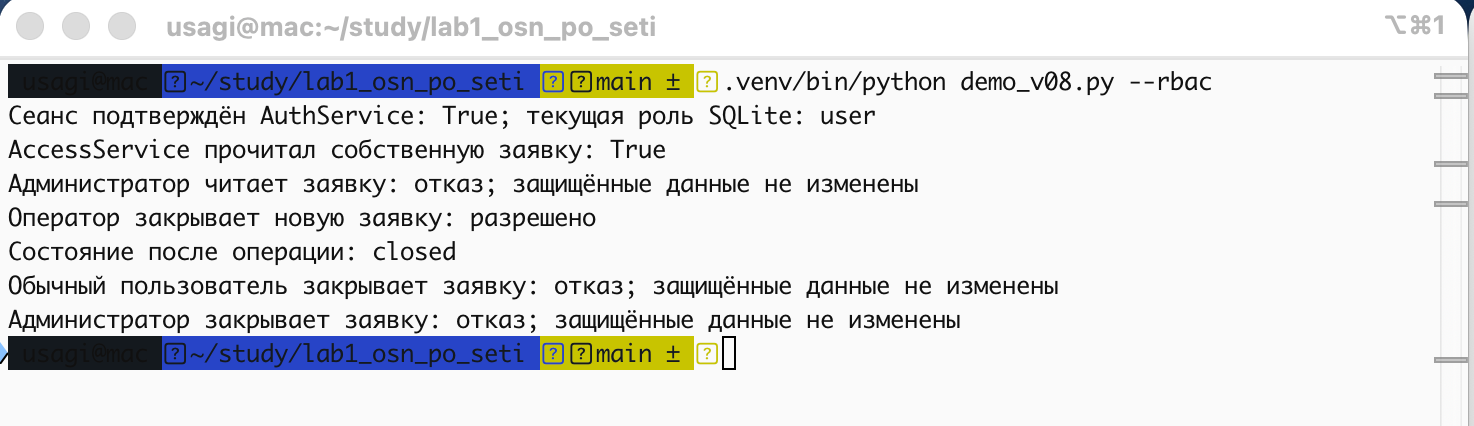
\includegraphics[width=\linewidth,height=5.4cm,keepaspectratio]{reports/lab8/screenshots_manual/lab8_03_functional_permissions.png}
\caption{Функциональные разрешения operator, user и admin.}
\end{figure}
\begin{figure}[H]
\centering
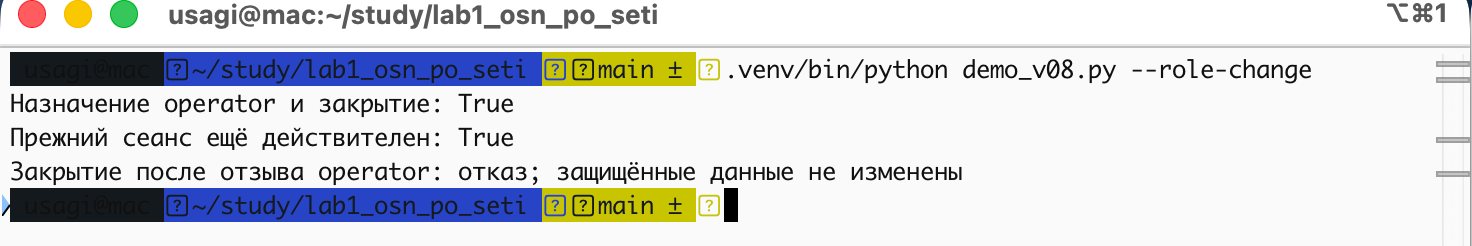
\includegraphics[width=\linewidth,height=5.4cm,keepaspectratio]{reports/lab8/screenshots_manual/lab8_04_role_change.png}
\caption{Отзыв роли operator применяется при следующем обращении с тем же сеансом.}
\end{figure}
\begin{figure}[H]
\centering
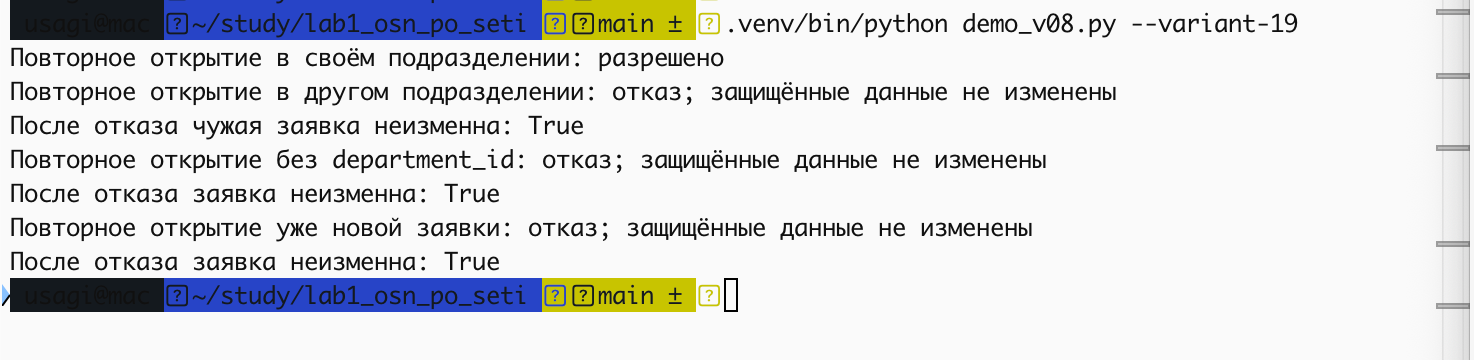
\includegraphics[width=\linewidth,height=5.4cm,keepaspectratio]{reports/lab8/screenshots_manual/lab8_05_variant19_allowed.png}
\caption{Вариант 19: специалист повторно открывает заявку своего подразделения.}
\end{figure}
\begin{figure}[H]
\centering
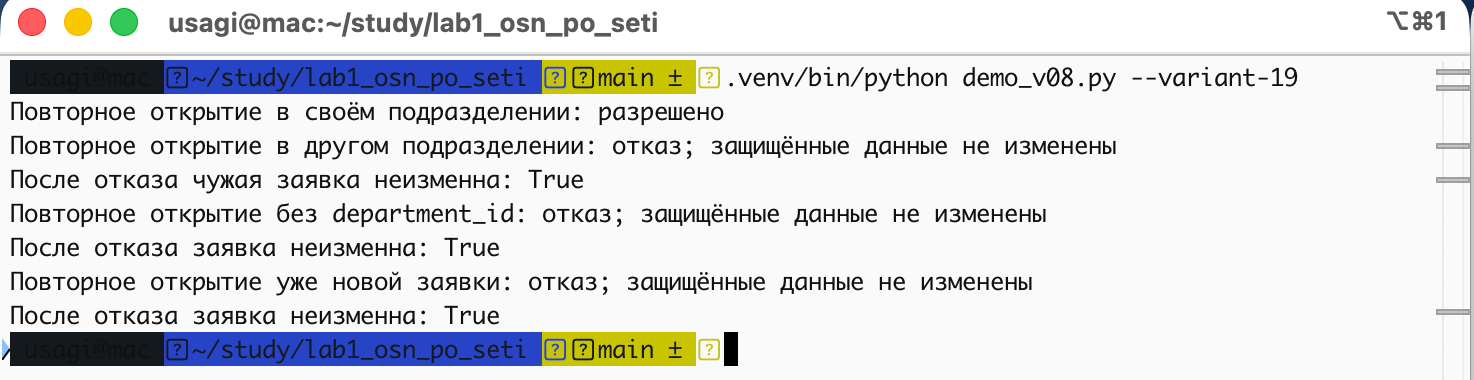
\includegraphics[width=\linewidth,height=5.4cm,keepaspectratio]{reports/lab8/screenshots_manual/lab8_06_variant19_denials.png}
\caption{Вариант 19: чужое подразделение, отсутствующий отдел и недопустимое состояние отклоняются без изменений.}
\end{figure}
\begin{figure}[H]
\centering
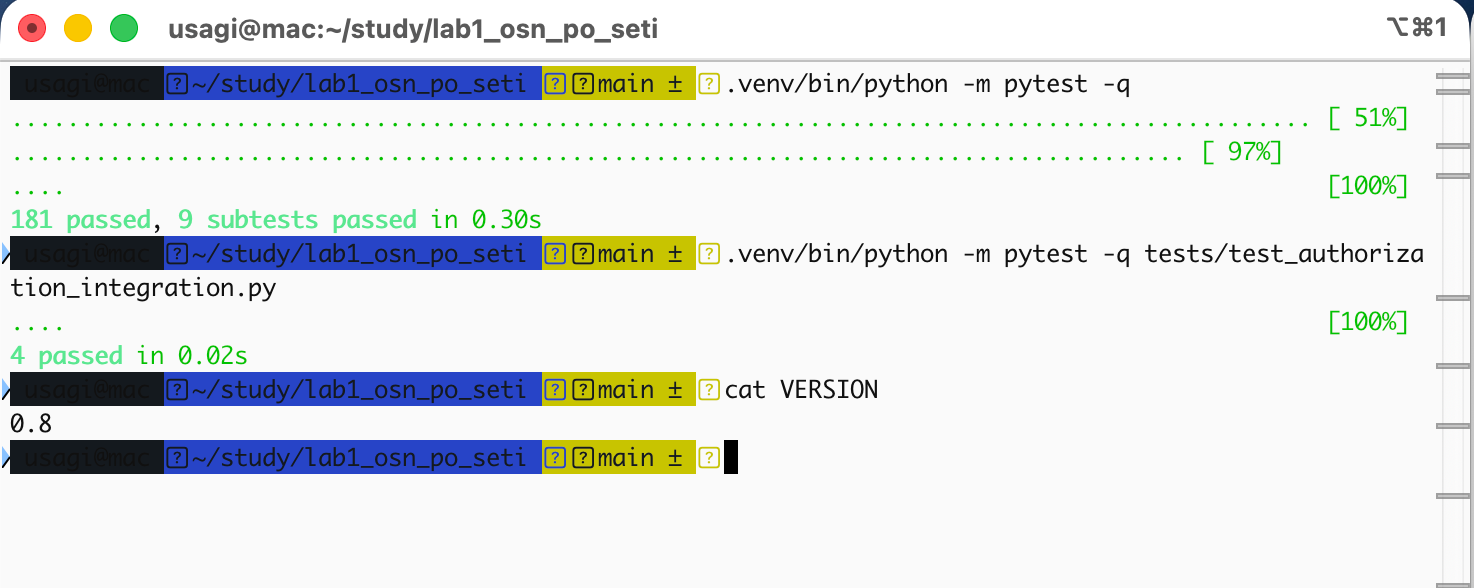
\includegraphics[width=\linewidth,height=5.4cm,keepaspectratio]{reports/lab8/screenshots_manual/lab8_07_tests_version.png}
\caption{Полный набор тестов, интеграционные проверки и значение VERSION 0.8.}
\end{figure}

\section{Вывод}
В v0.8 добавлен \texttt{AccessService}, который подтверждает пользовательский сеанс существующим AuthService, читает актуальные разрешения из общей SQLite-БД и проверяет права на объект. Миграции аддитивны и повторяемы; прежние неизвестные владельцы/отделы не придумываются. Пройдены 20 базовых тестов, восемь дополнительных тестов варианта 19, четыре интеграционные проверки и полный набор из 181 теста с 9 subtests. В отчёт включены семь настоящих терминальных снимков.

\section{Ответы на контрольные вопросы}
\begin{enumerate}
\item Действующий сеанс устанавливает личность, но не решает, имеет ли субъект право на любую конкретную заявку; дополнительно проверяются функция и объект.
\item \texttt{request.read} отвечает за доступность функции чтения роли. Проверка владельца сопоставляет подтверждённый ID с владельцем конкретной строки.
\item Клиентский \texttt{role} можно подменить; сервер загружает текущую роль из доверенной SQLite-записи.
\item Матрица выдаёт admin только \texttt{role.assign}. Принцип минимальных полномочий не даёт ему автоматическое чтение заявок.
\item Сеанс хранит идентичность, а роль повторно загружается при каждом обращении; потому следующий запрос использует уже обновлённую роль.
\item Отказ авторизации означает отсутствие полномочий. Недопустимый переход означает, что право на функцию есть, но текущий объект/статус не допускает переход; оба случая не меняют запись.
\item Параметризация отделяет данные от SQL-синтаксиса, но не проверяет, кому принадлежит строка. Нужна отдельная объектная проверка.
\item Для нескольких ролей потребуются таблицы назначения user-role и role-permission, правила объединения/запрета конфликтующих разрешений, миграция, обновлённая модель сессии и тесты жизненного цикла; их нельзя добавлять простым наследованием в текущую политику.
\end{enumerate}

\section{Список источников}
\begin{enumerate}
\item Методические указания «Практическая работа №8. Реализация ролевого управления доступом». 14 с. Материал, предоставленный для задания.
\item OWASP Foundation. Authorization Cheat Sheet. URL: \url{https://cheatsheetseries.owasp.org/cheatsheets/Authorization_Cheat_Sheet.html} (дата обращения: 29.10.2026).
\item OWASP Foundation. API1:2023 Broken Object Level Authorization. URL: \url{https://api-security.owasp.org/editions/2023/en/0xa1-broken-object-level-authorization/} (дата обращения: 29.10.2026).
\item Python Software Foundation. sqlite3 — DB-API 2.0 interface for SQLite databases. URL: \url{https://docs.python.org/3/library/sqlite3.html} (дата обращения: 29.10.2026).
\item NIST CSRC. Role-based access control (RBAC), Glossary. URL: \url{https://csrc.nist.gov/glossary/term/role_based_access_control} (дата обращения: 29.10.2026).
\end{enumerate}

\end{document}
